This chapter assumes that you have Traverso \Version\ or later installed on your system. If not yet so, please refer to chapter \ref{sect_installation} for instructions on how to install the programme.

Start Traverso from the application menu, or by hitting Alt+F2 and entering \texttt{traverso} in the command dialog. The first thing you will see is a file dialog asking you for the project directory. If you don't have one yet, create a new one. This directory will contain all projects, including the audio files. So be aware that if you want to do some serious audio work, you will need \emph{lots} of hard disk space. Change into the directory and press OK. After confirming your selection, the Traverso main window will be shown. It contains different regions which are sensitive for soft selections. The nomenclature used in this manual is shown in \FigT\ \ref{fig_gui01}.

\begin{figure}
 \centering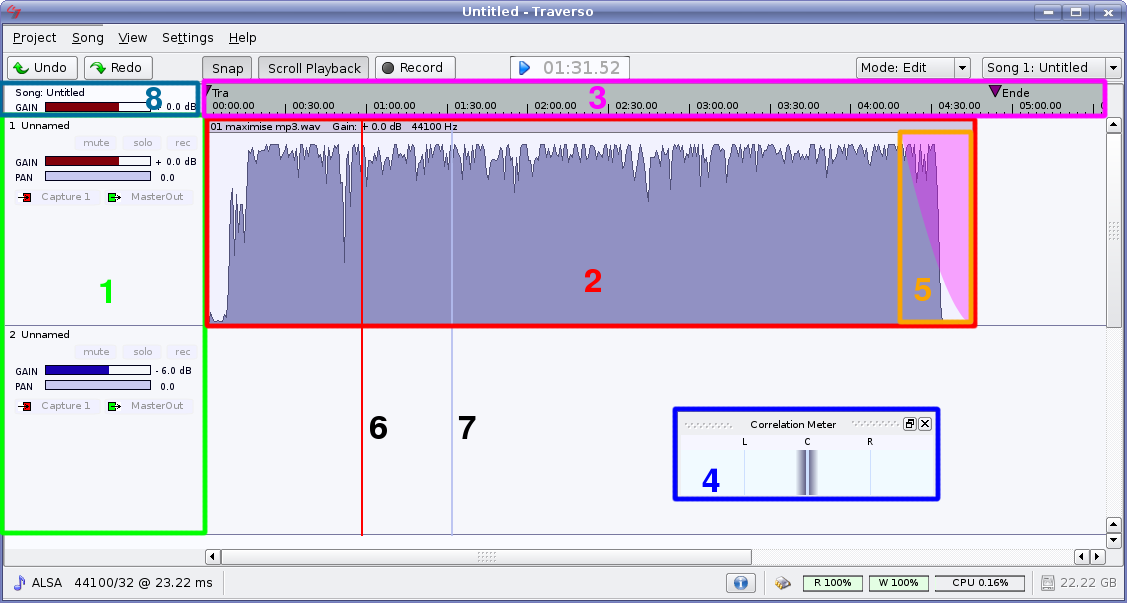
\includegraphics[width=\textwidth]{images/sshot06.png}
 \caption{Interface elements of Traverso: 1 Track panel: If the mouse cursor is hovering over this area, all key actions apply to the track beneath it; 2 Audio clip: Key actions apply to the audio clip; 3 Time line: Key actions apply to markers in the time line; 4 Dock window / Dock widget; 5 Fade out; 6 Work cursor; 7 Play head; 8 Sheet area.}
 \label{fig_gui01}
\end{figure}

Traverso uses dock windows for its tool dialogs, which allows to re-arrange the layout to your own liking. Just grab each one by the title bar and drag it to a new position. You can even stack the dock widgets on top of each other or detach from the main window and move freely. The latter is particularly handy with dual-screen setups, for the main window can occupy one screen, and the dock windows can be moved to the second screen (\FigB\ \ref{fig_mainwin02}).

\begin{figure}
 \centering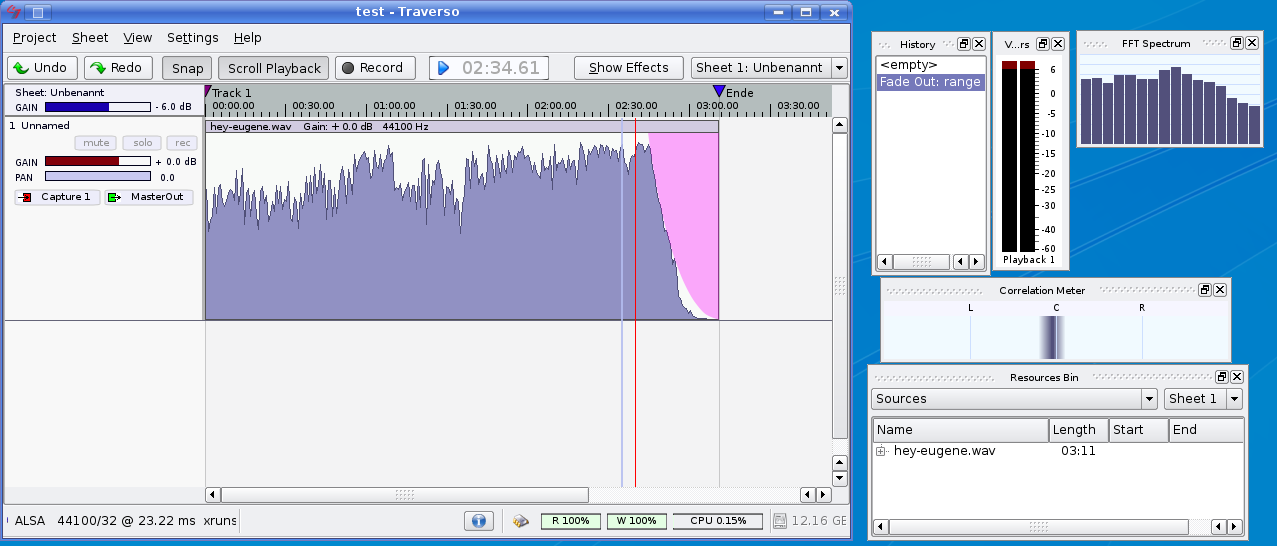
\includegraphics[width=\textwidth]{images/sshot03.png}
 \caption{The dock windows can also be detached from the main window and moved to the second screen in a multi-screen setup.}
 \label{fig_mainwin02}
\end{figure}

\section{The Driver Backend}
Four driver backends are supported to date: The Null driver, ALSA, the jack soundserver, and Port Audio (on Windows and Mac OS X). Let's have a look at all of them, what the advantages and disadvantages are, and how to set them up correctly. The currently loaded driver is displayed in the menu bar.

\subsection{Null Driver}

\includegraphics[height=\baselineskip]{images/tux.png}

\includegraphics[height=\baselineskip]{images/mac.png}

\includegraphics[height=\baselineskip]{images/win.png}
\\
The Null driver is a fallback solution which is set if no other driver is available, but you won't hear any output as long as the Null Driver is loaded. Hence there's hardly a situation where you want to load it manually. To select a valid driver, click on the \emph{Null Driver} label in the menu bar to open a configuration dialog (\FigB\ \ref{fig_driverconf}).

\subsection{ALSA}

\includegraphics[height=\baselineskip]{images/tux.png}
\\
If ALSA is selected, Traverso communicates directly with the ALSA layer, which is only possible if no other application occupies the sound system. So before selecting ALSA as your driver, make sure you stop playback of all other sound applications. Also check the KDE/Gnome system tray for minimized instances of amarok, XMMS, etc. Back in Traverso's driver configuration dialog set the driver to \emph{ALSA}, the rate to 44100, and leave the latency. Then press \emph{OK} and check if the entry in the menu bar has switched to \emph{ALSA}. If it refuses to load the new driver, your sound card may still be occupied by another application, so check again if you correctly stopped all multimedia applications and make sure that the sound daemon (e.\,g. aRTs) shuts down automatically when not used. Then try again to set the driver to ALSA. If it was accepted as a valid driver, the sound driver is set up correctly.

\subsection{Jack}

\includegraphics[height=\baselineskip]{images/tux.png}

\includegraphics[height=\baselineskip]{images/mac.png}
\\
Traverso can also connect to the jack soundserver, which provides advanced routing features and zero-latency connections between clients. If you don't want to use these features and ALSA works for you, there's no advantage in using jack. We recommend to use \emph{qjackctl}, which allows to easily setup jack for your system. Start the jack daemon by pressing \emph{Start} in qjackctl. When it is running, set the driver in Traverso's configuration dialog (\FigB\ \ref{fig_driverconf}) to \emph{jack} and press \emph{OK}. The menu bar should display \emph{jack} if the driver was loaded correctly. Now go back to qjackctl and open the \emph{Connect} dialog. \emph{Important:} You must set up the connection manually, otherwise you won't hear any sound. Select the Traverso entry in the left part (``Readable Clients''), and alsa\_pcm in the right part (``Writable Clients''), then press \emph{connect}. If a line connecting the two clients is drawn, the sound system is set up correctly.

\begin{figure}
 \centering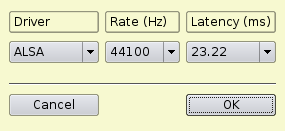
\includegraphics[width=0.5\textwidth]{images/sshot02.png}
 \caption{The audio driver backend can be selected from the menu bar. Traverso supports ALSA, jack, and PortAudio, and has a \emph{Null Driver} as fallback solution if no working driver is available.}
 \label{fig_driverconf}
\end{figure}

\subsection{Port Audio}

\includegraphics[height=\baselineskip]{images/mac.png}

\includegraphics[height=\baselineskip]{images/win.png}
\\
Port audio is the recommended driver backend on Mac OS X and Microsoft Windows. It connects to the system's native sound system (CoreAudio on OS X, WMME on Windows). Simply select ``PortAudio'' in the driver configuration widget, the samplerate you wish to use, and a latency that works for you.

\section{Recording file format}
From the menu ``Settings $\rightarrow$ Recording file format'' you can set the file format used for recorded audio. \emph{Wave} has been the standard audio format in the computer world for years. It is uncompressed, and Traverso stores all audio data in 32~bit floating point precision, no matter what bit depth the driver backend was set to. Wave files, however, are limited to a size of 2~GB. For a mono recording in 44100~Hz 32~bit resolution this gives a maximum recording time of approximately 3 hours and 20 minutes. For a stereo recording it is only half of that time. If you plan to record longer you should use the \emph{Wave-64} format instead, which can write much larger files. The third format, \emph{WavPack}, uses a lossless compression algorithm to shrink your files without affecting the quality of the audio data. However, since the encoding is done in real time, more CPU power is required while recording. If you are short of disk space but have a decent CPU, this format is certainly a good choice.
